% sections/results.tex
\chapter{Risultati}\label{chap:results}
 
Questo capitolo presenta i risultati ottenuti applicando la pipeline descritta nel
Capitolo~\ref{chap:methodology} al dataset AIS delle Hawaii.
I risultati sono organizzati in quattro sezioni: la prima descrive il dataset nelle
sue dimensioni finali dopo il pre-processing; la seconda mostra i risultati qualitativi
prodotti dalla fase di Knowledge Discovery; la terza riporta i risultati quantitativi
della fase di anomaly detection; la quarta ne discute l'interpretazione e le implicazioni.
 
% ─────────────────────────────────────────────
\section{Dataset}\label{sec:res_dataset}
 
Il dataset utilizzato comprende i messaggi AIS ricevuti dal NOAA nel primo trimestre
del 2019 (gennaio-marzo inclusi), filtrati sull'area geografica delle Hawaii tramite
la bounding box descritta nella Sezione~\ref{sec:meth_dataset}.
 
\subsection{Dimensioni e composizione}
 
I dati grezzi, dopo il filtraggio geografico, ammontano a 5.462.415 record. A seguito
della rimozione dei duplicati esatti il dataset si riduce a 5.460.800 record, generati
da 602 imbarcazioni distinte (in media 9.071 record per nave, con un minimo di 1 e un
massimo di 82.554).
 
L'applicazione della soglia dinamica sull'attività delle imbarcazioni
(Sezione~\ref{sec:meth_preprocessing}), pari al 10\% del numero medio di record per
nave e quindi a 907 record, ha eliminato 199 imbarcazioni, corrispondenti allo 0,84\%
dei record totali. Il dataset risultante conta 5.415.168 record relativi a 403
imbarcazioni, sulle quali si osservano le seguenti statistiche sul numero di record per
nave: media di 13.437 record, deviazione standard di 16.309, con un massimo di 82.554 e
un minimo di 921 record per singola imbarcazione.
 
Dopo la fase di ottimizzazione della memoria, il dataset è passato da circa 702~MB a
circa 465~MB, con un risparmio prossimo al 34\%.
 
\subsection{Classificazione degli stati e punti stazionari}
 
Nella fase di classificazione degli stati di navigazione, 7 record sono stati rimossi
in quanto associati a velocità istantanee non plausibili (superiori a 102 nodi),
portando il dataset a 5.415.156 record complessivi. Di questi, 3.766.844 punti sono
stati classificati come stazionari (comprendendo gli stati \emph{stationary},
\emph{entry} ed \emph{exit}), e costituiscono l'insieme di partenza per la fase di
Knowledge Discovery. L'aggregazione di questi punti per coordinate ha prodotto
51.801 coppie di coordinate distinte.
 
\subsection{Waypoint e rotte estratte}
 
Il clustering H-DBSCAN applicato ai punti stazionari aggregati ha identificato
144 waypoint distinti (da \texttt{WP\_0} a \texttt{WP\_143}).
I punti che ricadono in più di un waypoint, a causa della sovrapposizione degli inviluppi
convessi, sono 7.298, pari allo 0,135\% del dataset: l'effetto della regola di assegnazione
descritta nella Sezione~\ref{ssec:meth_routes} è quindi trascurabile. A partire da questi waypoint,
sono state estratte in tutto 910 rotte distinte e 35.731 trip.
 
Per la fase di anomaly detection è stata selezionata la rotta \texttt{WP\_135 - WP\_118},
una delle più trafficate tra quelle estratte, percorsa da 40 imbarcazioni distinte
per un totale di 184 trip. La lunghezza dei trip (in numero di punti) presenta una
media di 110,0, una mediana di 95,5, un minimo di 41 e un massimo di 524 punti.
 
% ─────────────────────────────────────────────
\section{Risultati qualitativi}\label{sec:res_qualitative}
 
Questa sezione mostra gli output visivi prodotti dalla fase di Knowledge Discovery,
con l'obiettivo di verificare che i waypoint e le rotte estratte corrispondano a
strutture geograficamente coerenti con il traffico marittimo dell'arcipelago delle
Hawaii.
 
\subsection{Waypoint identificati}
 
Le Figure~\ref{fig:res_dbscan} e~\ref{fig:res_hdbscan} mostrano i cluster di punti
stazionari ottenuti rispettivamente con DBSCAN ($\varepsilon = 0.075$, $N_{\min} = 10$)
e con H-DBSCAN ($\text{min\_cluster\_size} = 30$, $\text{max\_cluster\_size} = 10\,000$),
con i parametri descritti nella Sezione~\ref{ssec:meth_clustering}. In entrambe le figure
i punti in blu sono quelli assegnati a un cluster, i punti bianchi sono quelli classificati
come rumore, e il contorno nero di ogni cluster è il relativo \emph{convex hull}, che
definisce l'area del waypoint. Il riquadro rosso è la bounding box dell'area di studio.
La scala di colore indica il peso di ciascuna coordinata aggregata, pari al logaritmo in
base 2 del numero di messaggi AIS che vi ricadono, arrotondato all'intero più vicino
(Sezione~\ref{ssec:meth_clustering}); si tratta quindi di una grandezza adimensionale.

\begin{figure}[htbp]
    \centering
    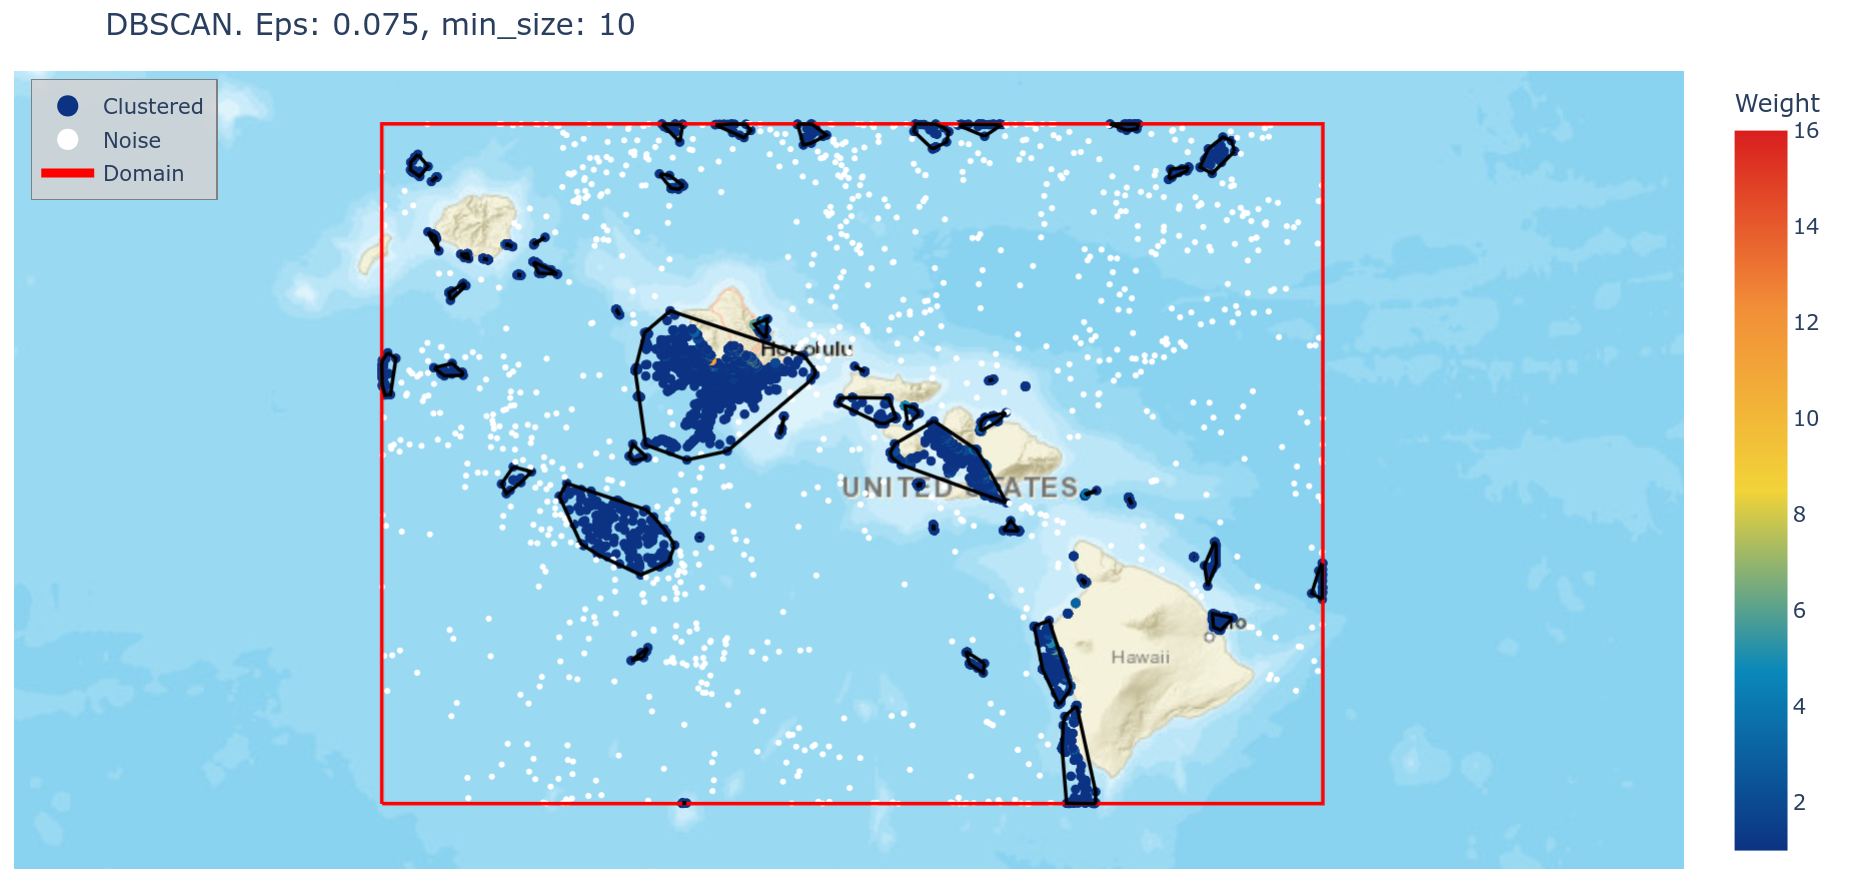
\includegraphics[width=\textwidth]{Results/DBSCAN.png}
    \caption{Waypoint identificati con DBSCAN ($\varepsilon = 0.075$, $N_{\min} = 10$).}\label{fig:res_dbscan}
\end{figure}

\begin{figure}[htbp]
    \centering
    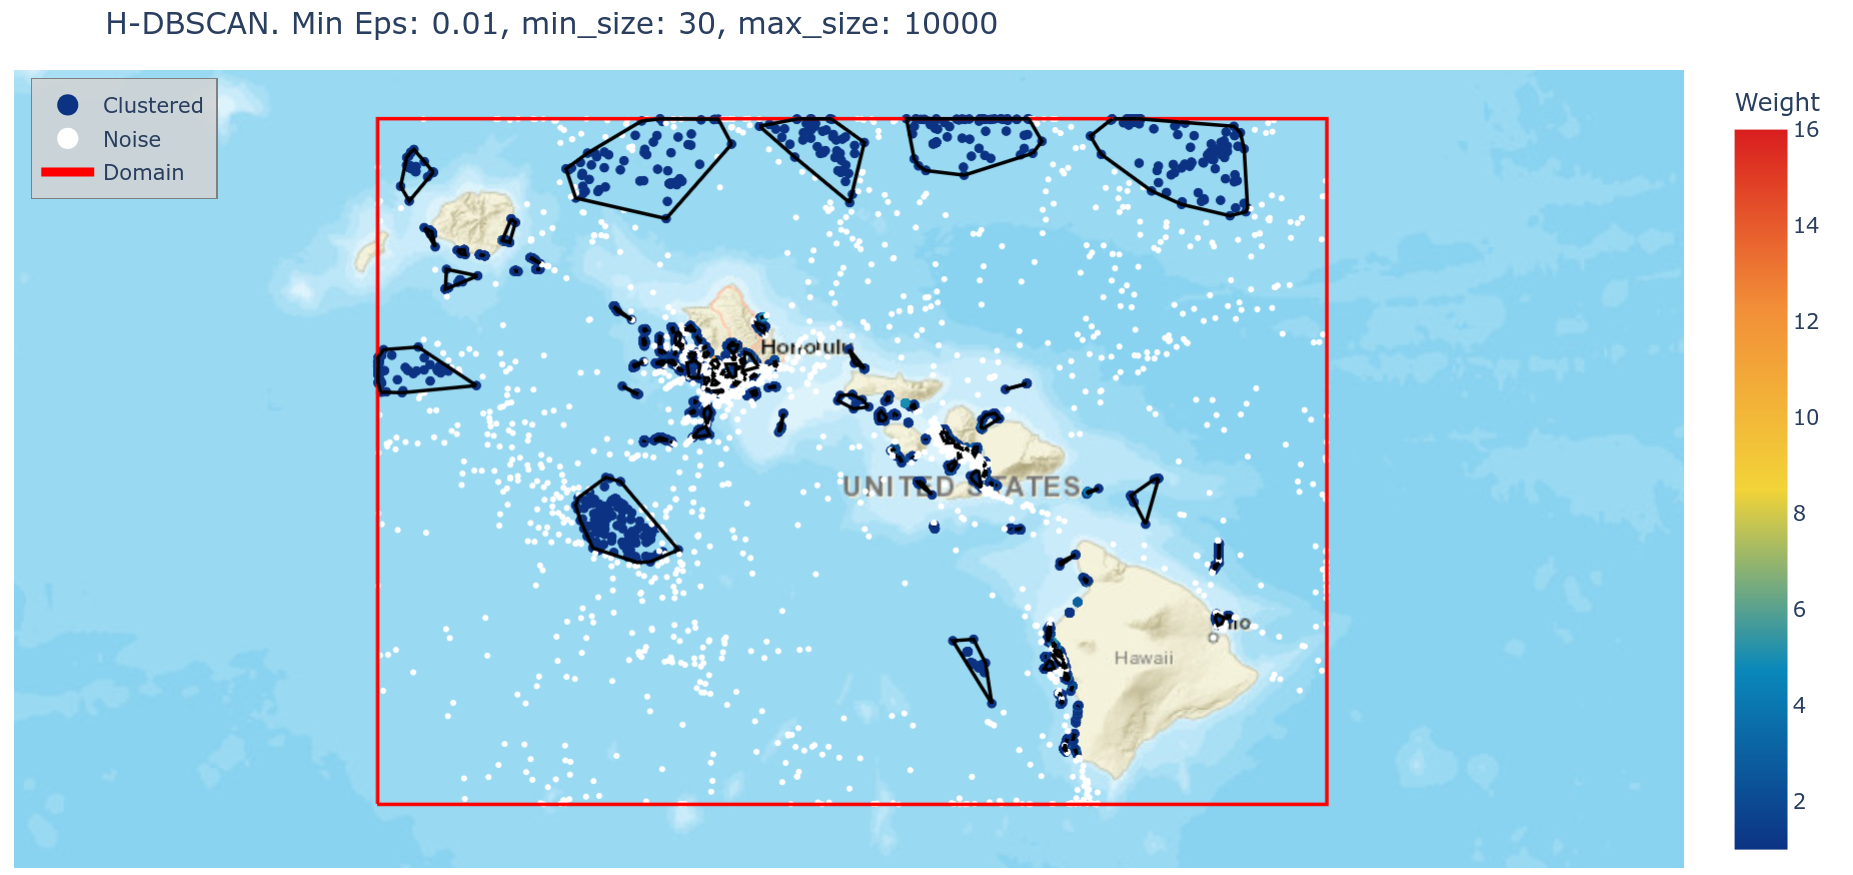
\includegraphics[width=\textwidth]{Results/H-DBSCAN.png}
    \caption{Waypoint identificati con H-DBSCAN ($\text{min\_cluster\_size} = 30$,
    $\text{max\_cluster\_size} = 10\,000$).}\label{fig:res_hdbscan}
\end{figure}

DBSCAN individua 55 cluster e classifica come rumore
1.001 delle 51.801 coordinate aggregate (1,93\%); H-DBSCAN, eseguito sulla tabella
espansa secondo i pesi (Sezione~\ref{ssec:meth_clustering}), individua 144 cluster e ne scarta 2.800 su 96.913
(2,89\%). Il confronto mette in evidenza il limite principale di DBSCAN con un raggio $\varepsilon$
fisso. Nell'area del porto di Honolulu e le zone di ancoraggio
vicine, la densità di punti stazionari è molto alta, e DBSCAN raggruppa tutta la zona in
un unico grande cluster che copre buona parte dell'isola. Lo stesso succede lungo la costa
occidentale dell'isola Maui e lungo la costa di Kona sull'isola di Hawaii, dove punti di sosta
distinti vengono fusi in poligoni allungati. Un waypoint di queste dimensioni non è utile
per l'estrazione delle rotte, perché fa coincidere in un solo nodo del grafo origini e
destinazioni che invece sono diverse.

H-DBSCAN, potendo adattarsi a densità locali diverse, scompone le stesse aree in molti
cluster più piccoli e compatti, che corrispondono in modo più plausibile a singoli porti,
moli e zone di ancoraggio. Nelle zone a bassa densità in mare aperto, invece, entrambi gli
algoritmi producono cluster di dimensioni simili (ad esempio il cluster a sud-ovest di Oahu
e quelli lungo il bordo settentrionale della bounding box). Per questo motivo H-DBSCAN è
stato adottato come approccio principale per le fasi successive della pipeline.

 
\subsection{Rotte estratte}
 
% PLACEHOLDER: inserire figura con la visualizzazione delle rotte estratte
% (grafo orientato waypoint → waypoint) sovrapposta alla mappa dell'arcipelago.
% Commentare le rotte principali emerse e la loro coerenza geografica.
 
\subsection{Trip sulla rotta selezionata}
 
% PLACEHOLDER: inserire figura con la visualizzazione dei 184 trip associati
% alla rotta selezionata WP_135 - WP_118.
 
% ─────────────────────────────────────────────
\section{Risultati quantitativi}\label{sec:res_quantitative}
 
\subsection{Parametri del modello Weibull}

I parametri della distribuzione di Weibull, stimati sull'intero insieme di 184 trip
della rotta selezionata (Sezione~\ref{sec:meth_anomaly}), risultano pari a
$m = 1{,}3105$ (coefficiente della relazione $\alpha = m \cdot \Delta t$ 
tra parametro di scala e intervallo temporale) e $\beta = 0{,}9358$ (parametro di forma medio).
 
% PLACEHOLDER: inserire grafico di fitting (shape/scale stimati sui vari lag
% temporali) a supporto dei valori riportati sopra.
 
\subsection{Anomaly scoring e ranking dei trip}
 
Applicando il modello ai 184 trip della rotta selezionata, i dieci trip con probabilità
combinata più alta (comportamento più regolare) sono, in ordine decrescente: i trip
23184, 24337, 23474, 8857, 11128, 14569, 8374, 15733, 25609 e 11307, con punteggi
compresi tra 3134,05 e 2534,98.
 
I dieci trip con probabilità combinata più bassa (candidati più probabili come
anomalie) sono, in ordine crescente di punteggio: il trip 3372 (211,39, il più
anomalo), seguito dai trip 3413, 3362, 10288, 30627, 10279, 24701, 7889, 30752
e 28433, con punteggi fino a 1196,21.
 
% PLACEHOLDER: inserire tabella riassuntiva con tutti i punteggi, e/o grafico
% della distribuzione dei punteggi sull'intera rotta.d
% PLACEHOLDER: inserire visualizzazione mappale dei trip con punteggio più
% basso sovrapposta a quella dei trip normali, per evidenziare visivamente
% le deviazioni.
 
\subsection{Metriche di valutazione}
 
% NOTA: le metriche quantitative non sono ancora state definite. Una volta
% stabilite, questa sottosezione dovrà riportare i valori ottenuti
% (es. AUC-ROC, precision/recall se disponibile un ground truth,
% oppure metriche interne come la separazione tra distribuzioni dei punteggi).
 
% ─────────────────────────────────────────────
\section{Interpretazione dei risultati}\label{sec:res_interpretation}
 
% PLACEHOLDER: questa sezione va scritta dopo aver ottenuto i risultati
% quantitativi. Di seguito alcune domande guida da affrontare:
%
% - I waypoint identificati corrispondono a porti, ancoraggi o punti di
%   passaggio noti dell'arcipelago? Ci sono waypoint inattesi?
% - Le rotte estratte riflettono le tratte commerciali o di traghetto
%   conosciute tra le isole?
% - I trip classificati come più anomali presentano caratteristiche
%   interpretabili (deviazioni spaziali, velocità inusuali, durate anomale)?
% - In che misura i risultati sono confrontabili con quelli riportati da
%   Pallotta et al. nel loro dataset originale (Stretto di Gibilterra,
%   Adriatico settentrionale)?
 
% ─────────────────────────────────────────────
\section{Sintesi}\label{sec:res_summary}
 
% PLACEHOLDER: scrivere dopo aver completato le sezioni precedenti.
% La sintesi dovrà riprendere brevemente i risultati principali e
% anticipare il Capitolo~\ref{chap:conclusions}, in cui verranno discusse
% le conclusioni generali e le possibili direzioni future.
